\newpage
\section{Problem 1: State (7 pts)}

\subsection{Description:}

The declaration of the state of the system is defined by

\begin{itemize}
    \item The set of phone numbers (call it \textit{numbers}) that are recorded in contacts
    \item A record of association between names and phone numbers, given by a correspondence
        (call it \textit{recorded}).
\end{itemize}

\begin{enumerate}
    \item Provide a diagram to visualize the state of the system.
    \item Provide a formal definition for numbers.
    \item Does \textit{recorded} have to be captured by a function? What requirements would a function
enforce? Explain in detail.
    \item What is the domain and the codomain of \textit{recorded}?
    \item What type of function should \textit{recorded} be (full or partial)? Explain in detail.
    \item Will \textit{recorded} be an injective, surjective, or bijective? Explain in detail.
    \item Provide a formal definition for \textit{recorded}.
\end{enumerate}

\subsection{Answer:}

\begin{enumerate}
    \item The following figure visualizes the state of the system:
        \begin{figure}[h]
        \centering
        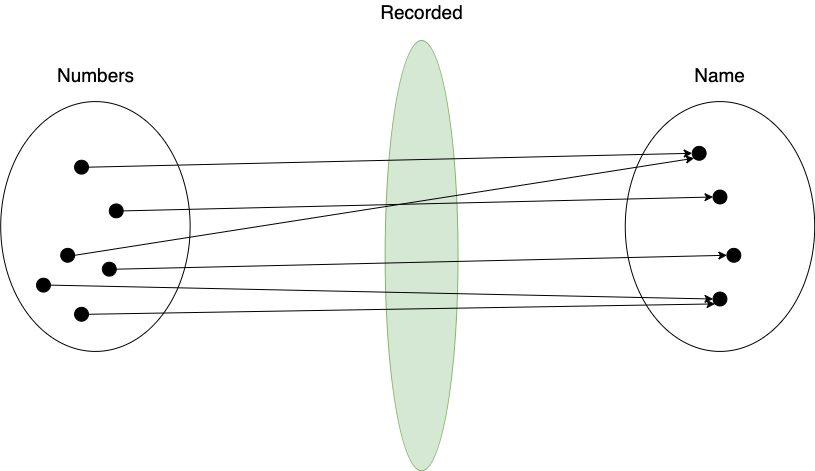
\includegraphics[scale=0.45]{images/Diagram.png}
        \caption{State of the System}
        \label{fig:Diagram}
        \end{figure}
    \item $numbers$ can be formally defined as: \\
    $\{ \forall x, y: numbers | (x \in numbers \wedge y \in numbers) \rightarrow x \neq y \}$
\item \emph{recorded} has to be a function since it is mapping 2 sets (\emph{NumberType} and \emph{NameType}). A function requires 2 sets A and B present and there exists assignments from elements in A to elements in B.
\item 
    \begin{itemize}
        \item[] Domain of \emph{recorded} is \emph{numbers}
        \item[] Codomain of \emph{recorded} is \emph{Name} (a subset of \emph{NameType}) = $\{a | a \in NameType \wedge \exists b \in NumberType \rightarrow \text{\emph{recorded(b)}} = a \}$
    \end{itemize}
    \item
    \item
    \item
\end{enumerate}
